\section{Two inequalities for polynomial multiplication}\hypertarget{p107.sec.4}{}
We apply the shared-leg inequality to polynomial multiplication, whose tensor rank is explicit. For positive integers $a,b$, let
\begin{equation}
C(a,b)=\sum_{i=0}^{a-1}\sum_{j=0}^{b-1}x_i y_j z_{i+j}.\tag{4.1}\hypertarget{p107.eq.4.1}{}
\end{equation}
This is multiplication of homogeneous binary forms of degrees $a-1$ and $b-1$, paired with the dual of the output space. Evaluation at $a+b-1$ distinct points followed by interpolation gives $\mathrm R(C(a,b))\le a+b-1$. Its output flattening has rank $a+b-1$, since every output monomial is a product of input monomials. Hence
\begin{equation}
\mathrm R(C(a,b))=a+b-1.\tag{4.2}\hypertarget{p107.eq.4.2}{}
\end{equation}
Fix a character $\lambda$, put $t=(p_X+p_Y+p_Z)/3>0$, and let $\lambda_\pi(A)$ denote its value after permuting the legs of $A$ by $\pi\in S_3$. Each $\lambda_\pi$ is again a character; denote its first-leg dot-product exponent by $p_X^{(\pi)}$. Each of the three original exponents occurs twice, so
\begin{equation}
\sum_{\pi\in S_3}p_X^{(\pi)}=2(p_X+p_Y+p_Z)=6t.\tag{4.3}\hypertarget{p107.eq.4.3}{}
\end{equation}
Products over permuted legs are used in tensor-power arguments \cite[Appendix A.3 of the full version]{r10}. Here we take all six permutations, so each original leg occurs equally often in each position, and define the \emph{symmetrized profile}
\begin{equation}
P(a,b)=\left(\prod_{\pi\in S_3}\lambda_\pi(C(a,b))\right)^{1/(6t)}.\tag{4.4}\hypertarget{p107.eq.4.4}{}
\end{equation}
Exchanging the input legs permutes the factors, while $C(1,b)=B_X(b)$ determines the boundary values. These identities, \hyperlink{p107.eq.4.2}{(4.2)}, and \hyperlink{p107.eq.4.3}{(4.3)} give
\begin{equation}
P(a,b)=P(b,a)>0,\qquad P(1,b)=b,\qquad P(a,b)\le(a+b-1)^{1/t}.\tag{4.5}\hypertarget{p107.eq.4.5}{}
\end{equation}
The next two lemmas show that successive increments of $P$ in either argument are nonincreasing, and that, with the first argument $a$ fixed, replacing the second argument $h$ by $3h+a-1$ increases the value at least threefold. \hyperlink{p107.result.5.1}{Lemma 5.1} will use these two constraints to force growth along the diagonal, which can then be compared with the rank bound in \hyperlink{p107.eq.4.5}{(4.5)}.

\subsection{A determinant filtration}\hypertarget{p107.sec.4.1}{}
Tensoring with $B_X(2)$ doubles the second-input and output spaces. Multiplication on a quotient and a kernel of these spaces will produce the neighboring input lengths $b+1$ and $b-1$. To obtain a degeneration of the whole tensor, the bases and weights must work for every first input.

\begin{result}{Lemma}{4.1}{Discrete concavity}
For $a\ge1$ and $b\ge2$,
\begin{equation}
2P(a,b)\ge P(a,b+1)+P(a,b-1).\tag{4.6}\hypertarget{p107.eq.4.6}{}
\end{equation}
By symmetry, the analogous inequality holds in the first argument.
\end{result}
\begin{amsthmproof}
Let $V_e$ be the degree-$e$ homogeneous forms in $u,v$, and set $W_1=\operatorname{span}(s,w)$ for a second pair of variables. The tensor $C(a,b)\otimes B_X(2)$ represents multiplication
\[
V_{a-1}\times(V_{b-1}\otimes W_1)\longrightarrow V_{a+b-2}\otimes W_1.
\]
Put $D=uw-vs$. For $e\ge1$, diagonal substitution $(s,w)=(u,v)$ gives the exact sequence
\begin{equation}
0\longrightarrow DV_{e-1}\longrightarrow V_e\otimes W_1\longrightarrow V_{e+1}\longrightarrow0.\tag{4.7}\hypertarget{p107.eq.4.7}{}
\end{equation}
Diagonal substitution is surjective on monomials, so its kernel has dimension $e$. That kernel contains $DV_{e-1}$, which also has dimension $e$ because multiplication by $D$ is injective. This proves exactness and gives the determinant exact sequence underlying the degree-one Clebsch--Gordan construction \cite[Section 2.6 of the author version]{r9}.

Choose quotient lifts $u^{e-i}v^i s$ for $0\le i\le e$, followed by $v^e w$, and append the kernel basis $Du^{e-1-j}v^j$ for $0\le j<e$. Their diagonal images and their kernel factors are the standard monomial bases. Fix these bases at degrees $b-1$ and $a+b-2$, independently of the first input. For every $f\in V_{a-1}$, multiplication commutes with diagonal substitution and sends $Dg$ to $D(fg)$. Thus all slices have the form
\begin{equation}
\begin{array}{r|cc}
 & \text{input quotient} & \text{input kernel}\\\hline
\text{output quotient} & M_f^+ & 0\\
\text{output kernel} & * & M_f^-
\end{array}\tag{4.8}\hypertarget{p107.eq.4.8}{}
\end{equation}
in these fixed bases. Here $M_f^+$ is multiplication $V_b\to V_{a+b-1}$, and $M_f^-$ is multiplication $V_{b-2}\to V_{a+b-3}$. In particular, the two diagonal tensor blocks are exactly $C(a,b+1)$ and $C(a,b-1)$.

In these bases, give weight zero to the first leg and to all quotient coordinates, weight $-1$ to the second-leg kernel coordinates, and weight $+1$ to the output-dual kernel coordinates. The only potentially negative block in \hyperlink{p107.eq.4.8}{(4.8)} is zero, while the block marked $*$ has weight $+1$ and disappears. The weight-zero tensor therefore consists of $C(a,b+1)$ and $C(a,b-1)$, with a common first leg and disjoint second and third legs. For example, when $a=b=2$, the identity $u(vw)=v^2s+vD$ shows that multiplication of a quotient lift can have both quotient and kernel components.

Applying degeneration monotonicity and \hyperlink{p107.result.3.2}{Corollary 3.2} to these two blocks, for any probability pair $q=(q_+,q_-)$ we obtain
\[
2^{p_X^{(\pi)}}\lambda_\pi(C(a,b))\ge e^{p_X^{(\pi)}H(q)}\lambda_\pi(C(a,b+1))^{q_+}\lambda_\pi(C(a,b-1))^{q_-}.
\]
Multiply all six inequalities at the same $q$ and take the power $1/(6t)$. By \hyperlink{p107.eq.4.3}{(4.3)}, this gives
\[
2P(a,b)\ge e^{H(q)}P(a,b+1)^{q_+}P(a,b-1)^{q_-}.
\]
For positive $A,B$, the maximum of $e^{H(q)}A^{q_+}B^{q_-}$ is $A+B$, attained at $q=(A,B)/(A+B)$. For positive $q_+,q_-$, this follows from the weighted arithmetic-geometric mean inequality applied to $A/q_+$ and $B/q_-$; the boundary follows by continuity. Taking this common maximizing pair proves \hyperlink{p107.eq.4.6}{(4.6)}.
\end{amsthmproof}

\FloatBarrier
\begin{figure}[!ht]
\centering
% Columns z=0,...,4; rows y=0,...,3, ordered downwards.
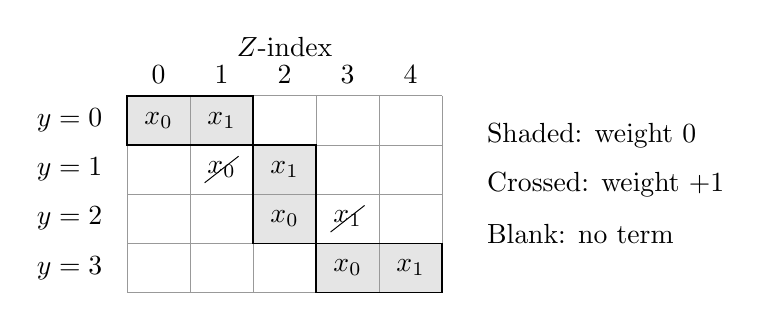
\begin{tikzpicture}[x=0.8cm,y=-0.625cm]
\fill[black!10] (0,0) rectangle (2,1);
\fill[black!10] (2,1) rectangle (3,3);
\fill[black!10] (3,3) rectangle (5,4);
\foreach \col in {0,...,5} {\draw[black!40,line width=0.25pt] (\col,0)--(\col,4);}
\foreach \row in {0,...,4} {\draw[black!40,line width=0.25pt] (0,\row)--(5,\row);}
\draw[black,line width=0.6pt] (0,0) rectangle (2,1);
\draw[black,line width=0.6pt] (2,1) rectangle (3,3);
\draw[black,line width=0.6pt] (3,3) rectangle (5,4);
\node at (2.5,-1.0) {$Z$-index};
\foreach \col in {0,...,4} {\node at (\col+0.5,-0.42) {$\col$};}
\foreach \row in {0,...,3} {\node[anchor=east] at (-0.24,\row+0.5) {$y=\row$};}
\node at (0.5,0.5) {$x_0$};
\node at (1.5,0.5) {$x_1$};
\node at (1.5,1.5) {$x_0$};
\node at (2.5,1.5) {$x_1$};
\node at (2.5,2.5) {$x_0$};
\node at (3.5,2.5) {$x_1$};
\node at (3.5,3.5) {$x_0$};
\node at (4.5,3.5) {$x_1$};
\draw[line width=0.35pt] (1.23,1.77)--(1.77,1.23);
\draw[line width=0.35pt] (3.23,2.77)--(3.77,2.23);
\node[anchor=west] at (5.56,0.80) {Shaded: weight $0$};
\node[anchor=west] at (5.56,1.80) {Crossed: weight $+1$};
\node[anchor=west] at (5.56,2.80) {Blank: no term};
\end{tikzpicture}

\caption{The degeneration of $C(2,4)$, with $a=2$, $h=1$. A cell $(y,z)$ contains $x_i$ when $z=y+i$. The three shaded blocks survive, and the two crossed terms disappear. The blocks have disjoint $Y$- and $Z$-coordinates but share $x_0,x_1$. The middle block is $C(2,1)$ with its second and third legs exchanged and its first-leg basis reversed.}
\hypertarget{p107.figure.1}{}\label{fig:107-sectors}
\end{figure}
\FloatBarrier

\subsection{Three sectors}\hypertarget{p107.sec.4.2}{}
\begin{result}{Lemma}{4.2}{Shifted tripling}
For all positive integers $a,h$,
\begin{equation}
P(a,3h+a-1)\ge3P(a,h).\tag{4.9}\hypertarget{p107.eq.4.9}{}
\end{equation}
\end{result}
\begin{amsthmproof}
Put $B=3h+a-1$. A supported term of $C(a,B)$ has indices $0\le x<a$, $0\le y<B$, and $z=x+y$. Partition the $Y$-indices and $Z$-indices as follows:
\[
\begin{array}{c|ccc}
 & \text{left} & \text{middle} & \text{right}\\\hline
Y & [0,h-1] & [h,2h+a-2] & [2h+a-1,3h+a-2]\\
Z & [0,h+a-2] & [h+a-1,2h+a-2] & [2h+a-1,3h+2a-3].
\end{array}
\]
Give weight $+1$ to middle $Y$-coordinates, weight $-1$ to middle $Z$-coordinates, and zero to all other coordinates. A left $Y$-index forces a left $Z$-index, because $x+y\le h+a-2$; a right $Y$-index forces a right $Z$-index. Thus no supported term has negative weight. The weight-zero part consists exactly of the three matched sectors. \hyperlink{p107.figure.1}{Figure 1} shows the smallest nontrivial example.

Translations identify the two outer branches with $C=C(a,h)$. The middle branch is
\[
\sum_{u=0}^{a-1}\sum_{r=0}^{h-1}x_{a-1-u}y_{h+u+r}z_{h+a-1+r}.
\]
It is $C$ with its second and third legs exchanged and its first-leg basis reversed. The reversal identifies this individual branch; no different first-leg maps are applied to the three branches of the whole tensor.

Let $\sigma$ exchange the second and third legs. The uniform probability vector on the three branches gives
\[
\lambda_\pi(C(a,B))\ge3^{p_X^{(\pi)}}\lambda_\pi(C)^{2/3}\lambda_\pi(C^\sigma)^{1/3}.
\]
Symmetrization removes the distinction between the ordinary and exchanged branches: composition with $\sigma$ permutes the six leg permutations. Thus $\prod_\pi\lambda_\pi(C^\sigma)=\prod_\pi\lambda_\pi(C)$. Multiplying the six inequalities and taking the power $1/(6t)$ proves \hyperlink{p107.eq.4.9}{(4.9)}.
\end{amsthmproof}
